\documentclass{article}

% Language setting
% Replace `english' with e.g. `spanish' to change the document language
\usepackage[german]{babel}

% Set page size and margins
% Replace `letterpaper' with `a4paper' for UK/EU standard size
\usepackage[letterpaper,top=2cm,bottom=2cm,left=3cm,right=3cm,marginparwidth=1.75cm]{geometry}

% Useful packages
\usepackage{amsmath}
\usepackage{graphicx}
\usepackage{subcaption} % Added package
\usepackage[colorlinks=true, allcolors=blue]{hyperref}

\title{Übungsprotokoll - NWT2 - Übung 03}
\author{\vspace{0.5cm} \Large VLANS\\ Thomas Brandstätter (s2210239002) \& Jakob Mayr (s2210239021)}

\begin{document}
\maketitle

\section{Konfiguration der Endsysteme}

In der folgenden Übung haben wir die PCs 4.1 und 4.2 benutzt, somit sind die Netze 4.x verwendet worden. Die IP-Konfiguration wird folgendermaßen vergeben: Klick auf „Network“ in der Taskleiste $\rightarrow$ „Network \& Internet Settings“ $\rightarrow$ „Change adapter options“ $\rightarrow$ gewünschtes Netzwerk Interface auswählen, in diesem Fall Ethernet 2 $\rightarrow$ „Properties“ $\rightarrow$ Doppelklick auf „Internet Protocol Version 4“ bzw. „Internet Protocol Version 6“. In den geöffneten Fenstern können wir nun jeweils die IP-Adresse, Subnetzmaske/Präfix und das Gateway eingeben. Folglich sind die Konfigurationen beider PCs zu sehen:

\begin{figure}[ht]
  \centering
  \subfigure[pc41 IPv4 config]{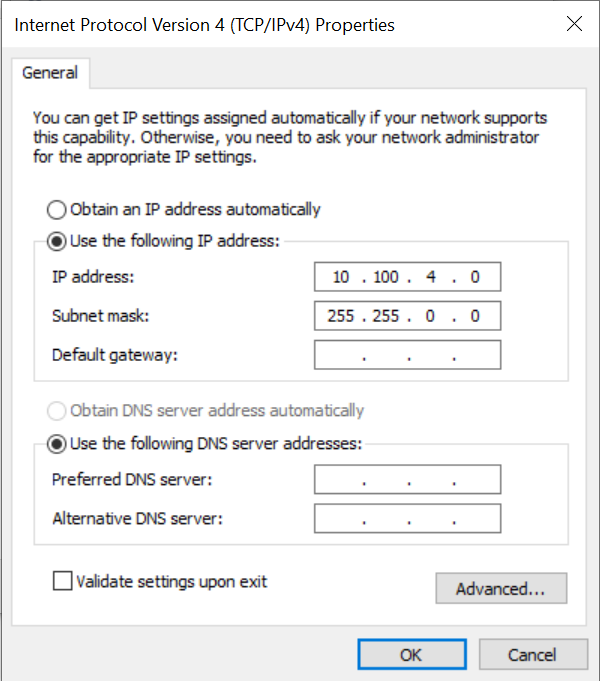
\includegraphics[width=0.2\textwidth]{Arbeitsergebnisse/PC41/pc41_IPv4_config.png}}
  \subfigure[pc41 IPv6 config]{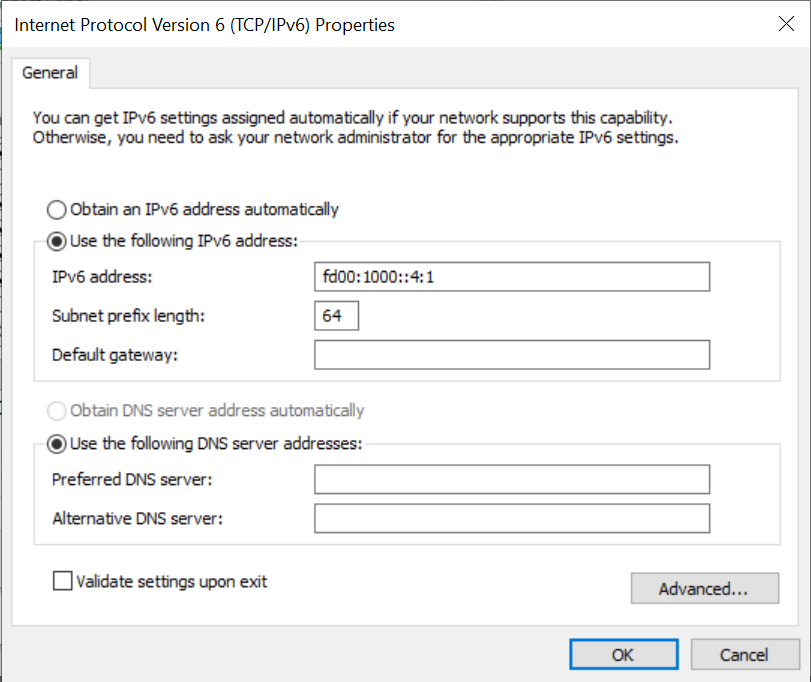
\includegraphics[width=0.2\textwidth]{Arbeitsergebnisse/PC41/pc41_IPv6_config.png}}
  \subfigure[pc42 IPv4 config]{\includegraphics[width=0.2\textwidth]{Arbeitsergebnisse/PC42/pc42_IPv4_config.png}}
  \subfigure[pc42 IPv6 config]{\includegraphics[width=0.2\textwidth]{Arbeitsergebnisse/PC42/pc42_IPv6_config.png}}
  \caption{Four Images}
  \label{fig:four_images}
\end{figure}

\section{Konfiguration der Gruppenswitches}

...

\subsection{Konfiguration der Gruppenrouter}

...

\subsection{Fragen zur Konfiguration}

...

\subsection{Tests und Interpretation ihrer Resultate}

...

\subsection{Konfiguration}

% \bibliographystyle{alpha}
% \bibliography{sample}

\end{document}

